\chapteropen{Chapter 9: Architecture and system design}{chapter-9}
\markboth{Ch. 9 | Architecture}{}


\begin{studycolumns}
\vspace{0pt}
\begin{eli5box}Architecture is a map of major parts and their communication. Choose the map using the case's important qualities and constraints.\end{eli5box}
\textbf{Answer check:} State the NFR, draw components/\allowbreak{}connectors, explain the mechanism, then name a cost or failure mode.
\needspace{326pt}
\subsection*{Visual: recognise the architectural organisation}
\sectionlabel{h-visual-recognise-the-architectural-organisation}
\par\smallskip\noindent\begin{minipage}{\linewidth}\centering
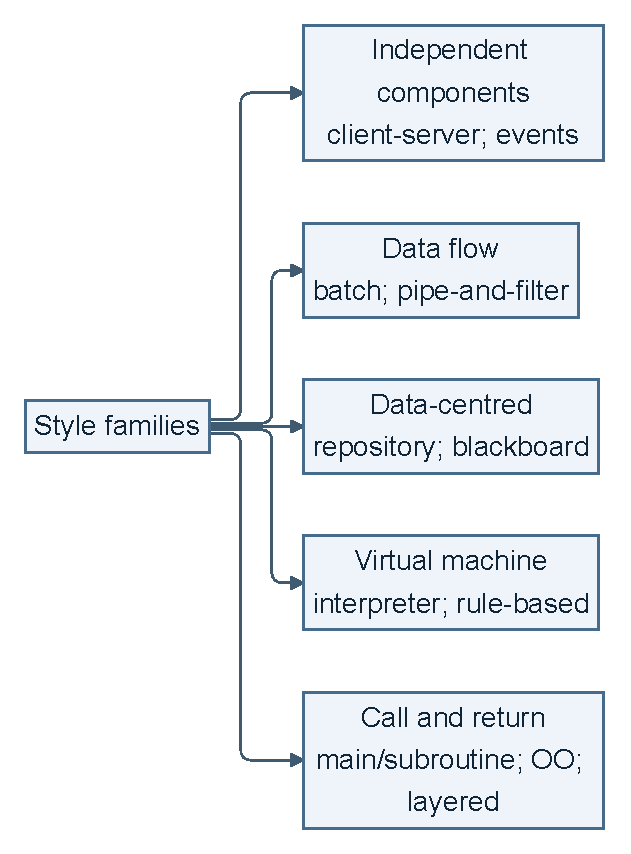
\includegraphics[width=185.38pt]{images/fig-024.pdf}
\captionof{figure}{recognise the architectural organisation}\end{minipage}\par\smallskip
\subsection*{9.1 Why design is hard here}
\sectionlabel{h-91-why-design-is-hard-here}
Scale, users, developers, versions, long lifetimes and changing technology increase complexity; cost, schedule, maintenance and NFRs constrain choices.
\subsection*{9.2 Definition}
\sectionlabel{h-92-definition}
\textbf{Architecture = components + connectors + constraints.} It abstracts implementation details, shows structure/\allowbreak{}interactions and demonstrates properties of interest. Connectors can be distributed across components rather than exist as separate runtime objects.
\end{studycolumns}


{\fontsize{9}{11}\selectfont
\begin{longtable}{L{\dimexpr 0.19355\linewidth-4.65pt\relax}L{\dimexpr 0.38710\linewidth-9.29pt\relax}L{\dimexpr 0.41935\linewidth-10.06pt\relax}}
\toprule
\rowcolor{ice}\textbf{} & \textbf{Definition} & \textbf{Examples} \\
\midrule\endfirsthead
\toprule\rowcolor{ice}\textbf{} & \textbf{Definition} & \textbf{Examples} \\
\midrule\endhead
\multicolumn{3}{r}{\scriptsize Continued on next page}\\\endfoot
\bottomrule\endlastfoot
\textbf{Component} & A unit of software that performs some function \textbf{at run time} & programs, objects, processes, clients, servers, databases \\
\textbf{Connector} & Interaction among components: communication, coordination or cooperation & shared variable access, procedure calls, RPC, communication protocols, data streams, transaction streams \\
\end{longtable}
}

\begin{studycolumns}
\vspace{0pt}
\subsection*{9.3 Architectural style}
\sectionlabel{h-93-architectural-style}
A style defines a family through component/\allowbreak{}connector vocabulary, composition constraints and semantic models. Instances can vary in count, interaction mechanism and component function. Event systems use implicit or explicit invocation; styles may coexist.
\subsection*{9.5 Layered architecture}
\sectionlabel{h-95-layered-architecture}
Upper layers call lower services. Benefits: abstraction, extension and lower-layer reuse. Costs: traversal overhead, difficult layer boundaries and poor fit for some systems. A direct lower-to-concrete-upper callback breaks the dependency direction; Observer abstracts that up-call.
\subsection*{9.6 Client--server}
\sectionlabel{h-96-clientserver}
Separate client/\allowbreak{}server computation supports concurrency, scalability, integration and change. Network protocols must handle delivery, failure and coordination; correctness is harder than a local call.
\subsection*{9.7 Pipe-and-filter}
\sectionlabel{h-97-pipe-and-filter}
Filters transform streams through pipes without shared state. Good for batch/\allowbreak{}stream transformations; weak for interactive shared-state behaviour.
\subsection*{9.8 Data-centred (repository /\allowbreak{} blackboard)}
\sectionlabel{h-98-data-centred-repository--blackboard}
Components communicate through a central repository/\allowbreak{}blackboard. It integrates independently changing producers/\allowbreak{}consumers, but creates shared coupling, contention and a potential single failure point.
\end{studycolumns}

\subsection*{9.9 Design principles (L12 and L14)}
\sectionlabel{h-99-design-principles-l12-and-l14}

{\fontsize{9}{11}\selectfont
\begin{longtable}{L{.27\linewidth}L{.66\linewidth}}
\toprule\rowcolor{ice}\textbf{Principle} & \textbf{Rule and failure check}\\\midrule\endhead
SRP /\allowbreak{} high cohesion & One reason to change; related responsibilities stay together. A God class or input parser that also writes the database fails this check.\\
OCP /\allowbreak{} identify variation & Encapsulate what varies; extend behind a stable contract. A type-switch scattered through clients forces modification.\\
Interfaces /\allowbreak{} low coupling & Depend on abstractions and minimise cross-module dependencies; avoid fields tied to concrete vendors.\\
DRY & Keep one authoritative representation of knowledge; duplicated creation logic is a warning.\\
Least Knowledge & Talk to immediate collaborators; avoid chains such as a.getB().getC().doIt().\\
Separation /\allowbreak{} modularity & Separate UI, rules and data; use abstraction and modular boundaries to support reuse. Business rules in event handlers defeat this.\\
Composition over inheritance & Assemble behaviour rather than grow fragile subclass hierarchies.\\\bottomrule
\end{longtable}}

\begin{studycolumns}
\vspace{0pt}

\needspace{321pt}
\subsection*{9.10 Design rationale frame (design rationale)}
\sectionlabel{h-910-design-rationale-frame-design-rationale}
\par\smallskip\noindent\begin{minipage}{\linewidth}\centering
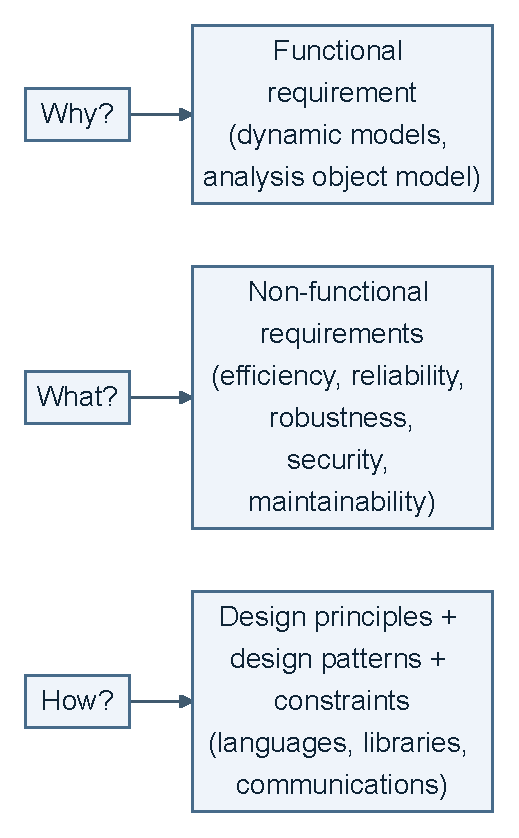
\includegraphics[width=152.26pt]{images/fig-025.pdf}
\captionof{figure}{9.10 Design rationale frame (design rationale)}\end{minipage}\par\smallskip
\par\needspace{65pt}\phantomsection\label{answer-architecture}
\textbf{Template A --- architecture justification:} [case NFR and why it matters]; [style, components and connectors]; [mechanism supporting the NFR]; [cost/\allowbreak{}failure mode and assumption]. Compare alternatives against the same requirement/\allowbreak{}workload; class or edge count alone is not quality evidence.
\subsection*{9.11 The design process (descriptive model)}
\sectionlabel{h-911-the-design-process-descriptive-model}
Model requirements; propose alternatives; validate against requirements; revise mismatches; elaborate, compare and select a blueprint.
\end{studycolumns}
